\documentclass[]{article}
\usepackage{lmodern}
\usepackage{amssymb,amsmath}
\usepackage{ifxetex,ifluatex}
\usepackage{fixltx2e} % provides \textsubscript
\ifnum 0\ifxetex 1\fi\ifluatex 1\fi=0 % if pdftex
  \usepackage[T1]{fontenc}
  \usepackage[utf8]{inputenc}
\else % if luatex or xelatex
  \ifxetex
    \usepackage{mathspec}
  \else
    \usepackage{fontspec}
  \fi
  \defaultfontfeatures{Ligatures=TeX,Scale=MatchLowercase}
\fi
% use upquote if available, for straight quotes in verbatim environments
\IfFileExists{upquote.sty}{\usepackage{upquote}}{}
% use microtype if available
\IfFileExists{microtype.sty}{%
\usepackage{microtype}
\UseMicrotypeSet[protrusion]{basicmath} % disable protrusion for tt fonts
}{}
\usepackage[margin=1in]{geometry}
\usepackage{hyperref}
\hypersetup{unicode=true,
            pdftitle={Singleton Error Experiments},
            pdfauthor={Andee Kaplan},
            pdfborder={0 0 0},
            breaklinks=true}
\urlstyle{same}  % don't use monospace font for urls
\usepackage{longtable,booktabs}
\usepackage{graphicx,grffile}
\makeatletter
\def\maxwidth{\ifdim\Gin@nat@width>\linewidth\linewidth\else\Gin@nat@width\fi}
\def\maxheight{\ifdim\Gin@nat@height>\textheight\textheight\else\Gin@nat@height\fi}
\makeatother
% Scale images if necessary, so that they will not overflow the page
% margins by default, and it is still possible to overwrite the defaults
% using explicit options in \includegraphics[width, height, ...]{}
\setkeys{Gin}{width=\maxwidth,height=\maxheight,keepaspectratio}
\IfFileExists{parskip.sty}{%
\usepackage{parskip}
}{% else
\setlength{\parindent}{0pt}
\setlength{\parskip}{6pt plus 2pt minus 1pt}
}
\setlength{\emergencystretch}{3em}  % prevent overfull lines
\providecommand{\tightlist}{%
  \setlength{\itemsep}{0pt}\setlength{\parskip}{0pt}}
\setcounter{secnumdepth}{5}
% Redefines (sub)paragraphs to behave more like sections
\ifx\paragraph\undefined\else
\let\oldparagraph\paragraph
\renewcommand{\paragraph}[1]{\oldparagraph{#1}\mbox{}}
\fi
\ifx\subparagraph\undefined\else
\let\oldsubparagraph\subparagraph
\renewcommand{\subparagraph}[1]{\oldsubparagraph{#1}\mbox{}}
\fi

%%% Use protect on footnotes to avoid problems with footnotes in titles
\let\rmarkdownfootnote\footnote%
\def\footnote{\protect\rmarkdownfootnote}

%%% Change title format to be more compact
\usepackage{titling}

% Create subtitle command for use in maketitle
\newcommand{\subtitle}[1]{
  \posttitle{
    \begin{center}\large#1\end{center}
    }
}

\setlength{\droptitle}{-2em}

  \title{Singleton Error Experiments}
    \pretitle{\vspace{\droptitle}\centering\huge}
  \posttitle{\par}
    \author{Andee Kaplan}
    \preauthor{\centering\large\emph}
  \postauthor{\par}
    \date{}
    \predate{}\postdate{}
  

\begin{document}
\maketitle

This is a set of small experiments with the goal of determining how
errors in the contingency table result in errors in the population size
estimate. We are interested ultimately in how errors from record linkage
are propagated through a capture-recapture method and result in biased
results. Specifically we will explore in two questions.

\begin{enumerate}
\def\labelenumi{\arabic{enumi}.}
\tightlist
\item
  Which type of errors are worse--errors in the number of records
  counted in only one database or errors in the number of records
  counted in multiple databases?
\item
  In a record linkage setting, at what point to singleton errors result
  in capture-recapture estimations of the population size that are no
  longer useful (coverage \(< 95\%\))
\end{enumerate}

\hypertarget{experiment-setup-and-data}{%
\section{Experiment Setup and Data}\label{experiment-setup-and-data}}

To set up our experiments, we start with a population of size
\(M = 1000\) and select with replacement to create \(D = 5\) databases
according to the inclusion probabilities in Table \ref{tab:inclusion}.
The inclusion probabilities were randomly generated from a
\(Beta(a_0, b_0)\) distribution. This results in \(n(0) = 262\) records
never having been recorded in any database, which is the value that we
will estimate using a capture-recapture procedure.

\begin{longtable}[]{@{}lrrrrr@{}}
\caption{\label{tab:inclusion}Inclusion probabilities for each of the
databases.}\tabularnewline
\toprule
& 1 & 2 & 3 & 4 & 5\tabularnewline
\midrule
\endfirsthead
\toprule
& 1 & 2 & 3 & 4 & 5\tabularnewline
\midrule
\endhead
inclusion & 0.1 & 0.2711 & 0.4202 & 0.0307 & 0.2953\tabularnewline
\bottomrule
\end{longtable}

To perform capture-recapture, I used the nonparametric latent class
model (NPLCM) of Manrique-Vallier (2016) with default priors and
hyperparameters. The posterior distribution of \(M\) is shown in Figure
\ref{fig:true-plot}, with the true value of \(M = 1000\) shown as a
vertical line. The posterior contains the true population size nicely,
indicating that in the absence of errors, the NPLCM model with default
priors and hyperparameters is working adequately.

\begin{figure}
\centering
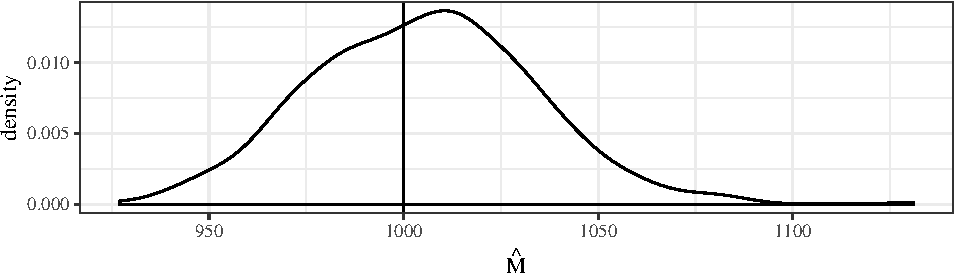
\includegraphics{singleton_errors_files/figure-latex/true-plot-1.pdf}
\caption{\label{fig:true-plot}The posterior distribution of \(M\) as
generated by the NPLCM, with the true value of \(M = 1000\) shown as a
vertical line. The posterior contains the true population size nicely,
indicating that in the absense of errors, the NPLCM model with default
priors and hyperparameters is working adequately.}
\end{figure}

\hypertarget{error-types}{%
\section{Error Types}\label{error-types}}

The first experiment we look at aims to answer the question, ``Which
type of errors are worse--errors in the number of records counted in
only one database or errors in the number of records counted in multiple
databases?''

In order to answer this, we will add or remove a fixed number, \(\rho\),
of records from random buckets in the \(2^D\) contingency table of the
captures. We will add or remove these records from the two types of
buckets, singleton or multiple inclusions, and compare the results of
running the NPLCM for capture-recapture to estimate \(M\). We look at
multiple values of \(\rho\) as different percentages of singletons from
\(5\%\) to \(50\%\). The result of this process is shown in Figure
\ref{fig:fixed-error-plots}. Because the process of introducing error is
random, we repeat it 100 times and look at the resulting 95\% credible
intervals for \(M\).

\begin{figure}
\centering
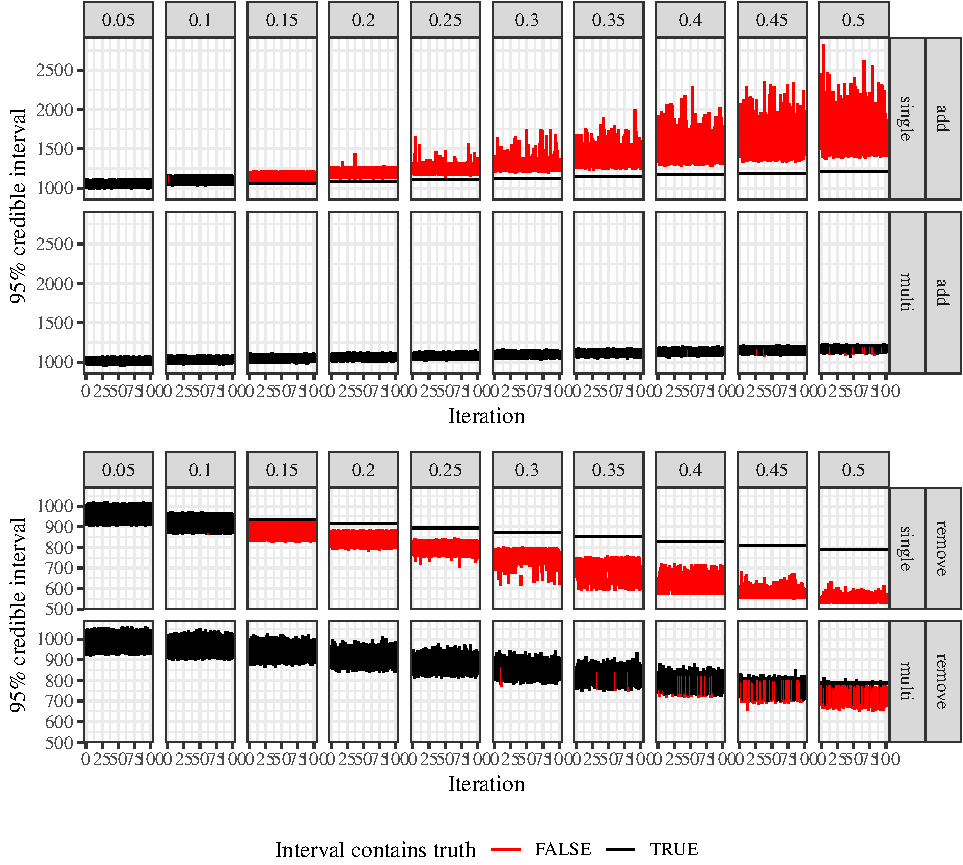
\includegraphics{singleton_errors_files/figure-latex/fixed-error-plots-1.pdf}
\caption{\label{fig:fixed-error-plots}The results of running the NPLCM
for capture-recapture to estimate \(M\) after adding and removing equal
numbers of singletons or multiple inclusions from the contingency table.
Because the process of introducing error is random, we repeat it100times
and look at the resulting 95\% credible intervals for \(M\). Errors that
are introduced to the singleton buckets in the contingency table have a
much greater effect on the estimate of \(M\) than do errors introduced
to the multiple inclusion buckets. This is shown by how many intervals
contain the true population size (black) versus those that do not (red).
For both adding and removing singletons, the estimates of \(M\) are
drastically different from reality between \(10\%\) and \(15\%\) error,
whereas for the multiples, an effect is not seen until much later.}
\end{figure}

Errors that are introduced to the singleton buckets in the contingency
table have a much greater effect on the estimate of \(M\) than do errors
introduced to the multiple inclusion buckets. This is shown by how many
intervals contain the true population size (black) versus those that do
not (red). For both adding and removing singletons, the estimates of
\(M\) are drastically different from reality between \(10\%\) and
\(15\%\) error, whereas for the multiples, an effect is not seen until
much later. This result indicates that errors in the singleton buckets
have a much higher impact on the capture-recapture method than errors in
the multiple inclusions. This could help us tailor a record linkage
method to work well for capture-recapture.

\hypertarget{record-linkage-setting}{%
\section{Record Linkage Setting}\label{record-linkage-setting}}

The experiments in Section \ref{error-types}, while informative, are not
realistic in terms of how errors occur in record linkage. In a record
linkage procedure, record will either be classified as singletons (no
linkage) or multiple inclusions (linked). The result is that errors in
singleton classification will necessarily also result in errors in
multiple inclusions. However, it is possible for a record linkage
procedure to correctly classify all the singletons, and still have a
high rate of overall error due to getting the actual linkage wrong.

In this second set of experiments, we are interested in exploring how
much singleton error from the record linkage procedure can the NPLCM
handle and still produce meaningful results. To test this, we once again
add or remove singletons according to \(\rho\), various proportions of
singletons from \(5\%\) to \(50\%\), but now we also add or remove those
records from randomly selected multiple inclusions buckets (in
accordance with a realistic record linkage scenario). The resulting 95\%
credible intervals are shown in Figures \ref{fig:rl-plot} and
\ref{fig:rl-zoom-plot} with intervals that contain the truth
\(M = 1000\) in black and those that do not in red.

\begin{figure}
\centering
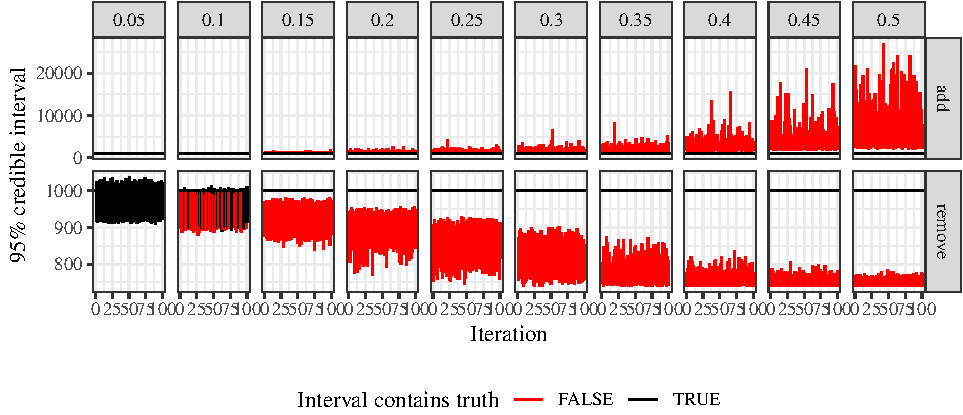
\includegraphics{singleton_errors_files/figure-latex/rl-plot-1.pdf}
\caption{\label{fig:rl-plot}95\% credible intervals resulting from the
NPLCM capture-recapture model after removing or adding various
proportions of singletons from \(5\%\) to \(50\%\) and in a record
linkage setting. Intervals that contain the truth \(M = 1000\) are shown
in black and those that do not in red. Somewhere between \(5\%\) and
\(10\%\) of singleton error leads to an unacceptable amount of error in
the estimation of \(M\) (coverage \textless{} 95\%).}
\end{figure}

Somewhere between \(5\%\) and \(10\%\) of singleton error leads to an
unacceptable amount of error in the estimation of \(M\) (coverage
\textless{} 95\%). We zoom in on these values in Figure
\ref{fig:rl-zoom-plot} to pinpoint how the errors are affecting coverage
in the posterior estimate of \(M\). This zoomed in view shows that
depending on if singletons are added (over linked) or removed (under
linked), the amount of acceptable error in singletons from the record
linkage procedure is around 5.5\% or 7.5\%, respectively. Tables
\ref{tab:rl-results} and \ref{tab:rl-zoom-results} display these results
numerically.

\begin{figure}
\centering
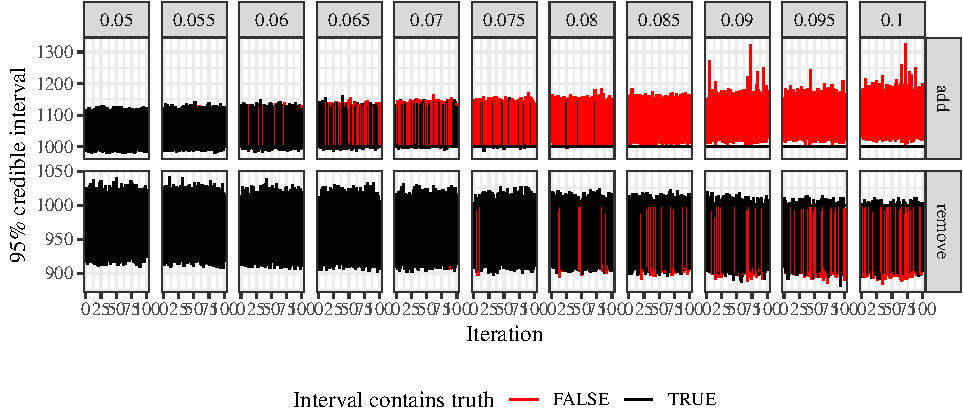
\includegraphics{singleton_errors_files/figure-latex/rl-zoom-plot-1.pdf}
\caption{\label{fig:rl-zoom-plot}95\% credible intervals resulting from
the NPLCM capture-recapture model after removing or adding various
proportions of singletons from \(5\%\) to \(10\%\) and in a record
linkage setting. Intervals that contain the truth \(M = 1000\) are shown
in black and those that do not in red. This zoomed in view shows that
depending on if singletons are added (over linked) or removed (under
linked), the amount of acceptable error in singletons from the record
linkage procedure is around 5.5\% or 7.5\%, respectively.}
\end{figure}

\begin{longtable}[]{@{}lrrrrrrrrrr@{}}
\caption{\label{tab:rl-results}Coverage of 95\% credible intervals for
\(M\) from using NPLCM capture-recapture after different error levels
are passed from the record linkage procedure. The amount of acceptable
error in singletons from the record linkage procedure is somewhere
between 5\% and 10\%.}\tabularnewline
\toprule
type & 0.05 & 0.1 & 0.15 & 0.2 & 0.25 & 0.3 & 0.35 & 0.4 & 0.45 &
0.5\tabularnewline
\midrule
\endfirsthead
\toprule
type & 0.05 & 0.1 & 0.15 & 0.2 & 0.25 & 0.3 & 0.35 & 0.4 & 0.45 &
0.5\tabularnewline
\midrule
\endhead
add & 1 & 0.00 & 0 & 0 & 0 & 0 & 0 & 0 & 0 & 0\tabularnewline
remove & 1 & 0.37 & 0 & 0 & 0 & 0 & 0 & 0 & 0 & 0\tabularnewline
\bottomrule
\end{longtable}

\begin{longtable}[]{@{}lrrrrrrrrrrr@{}}
\caption{\label{tab:rl-zoom-results}Coverage of 95\% credible intervals
for \(M\) from using NPLCM capture-recapture after different error
levels are passed from the record linkage procedure. Depending on if
singletons are added (over linked) or removed (under linked), the amount
of acceptable error in singletons from the record linkage procedure is
around 5.5\% or 7.5\%, respectively.}\tabularnewline
\toprule
type & 0.05 & 0.055 & 0.06 & 0.065 & 0.07 & 0.075 & 0.08 & 0.085 & 0.09
& 0.095 & 0.1\tabularnewline
\midrule
\endfirsthead
\toprule
type & 0.05 & 0.055 & 0.06 & 0.065 & 0.07 & 0.075 & 0.08 & 0.085 & 0.09
& 0.095 & 0.1\tabularnewline
\midrule
\endhead
add & 1 & 0.99 & 0.92 & 0.66 & 0.42 & 0.16 & 0.05 & 0.00 & 0.00 & 0.00 &
0.00\tabularnewline
remove & 1 & 1.00 & 1.00 & 1.00 & 0.98 & 0.98 & 0.91 & 0.83 & 0.77 &
0.67 & 0.56\tabularnewline
\bottomrule
\end{longtable}

\hypertarget{references}{%
\section*{References}\label{references}}
\addcontentsline{toc}{section}{References}

\hypertarget{refs}{}
\leavevmode\hypertarget{ref-manrique2016bayesian}{}%
Manrique-Vallier, Daniel. 2016. ``Bayesian Population Size Estimation
Using Dirichlet Process Mixtures.'' \emph{Biometrics} 72 (4). Wiley
Online Library: 1246--54.


\end{document}
